The research proposal of May 2025, reproduced below, set out to extend Wu et al.'s method to complex-valued nonlinear equations through a generalised \gls{qsvt}, and to add data-informed terms to its Hamiltonian. The order of the work changed once their examples had been reproduced and costed. The number of queries a preparation needs, whose growth with the resolution their Discussion leaves open, grows as a power of $N$, partly through a loose encoding of the dense differentiation matrix and partly through the norm that matrix gives the Hamiltonian (\Cref{sec:standard}). An extension to complex or nonlinear equations would inherit both costs, so the thesis first separates them, then reformulates the residual to lower the second, and only then carries both forms to coupled and nonlinear equations. \Cref{tab:proposal-deviations} records each deviation and its reason.

\begin{table}[htbp]
    \centering
    \caption[Deviations from the research proposal]{\textbf{The proposal's extensions were deferred until the method's cost was settled.} Each aim of the research proposal of May 2025, what the thesis did in its place, and why.}
    \label{tab:proposal-deviations}
    \small
    \begin{tabular}{@{}p{0.27\linewidth} p{0.33\linewidth} p{0.34\linewidth}@{}}
        \toprule
        Proposed & Outcome & Reason \\
        \midrule
        Extending \gls{qsvt} to the generalised construction for complex-valued, non-Hermitian operators & \Gls{gqsp} applies every filter, without a parity constraint. Complex-valued linear equations are carried by realification (R7) and Fourier bases on real ones (R9, R10); one natively complex encoding is built, and no complex residual is prepared (\Cref{sec:systems-complex}). & \Gls{gqsp} already lifts \gls{qsvt}'s restrictions to real coefficients and a definite parity. The filter acts only on the Hermitian $R^\dagger R$, so a complex or non-Hermitian residual needs no generalised transform. The cost had to be settled before any extension. \\
        \addlinespace
        Nonlinear \glspl{pde}: Burgers, nonlinear Schr\"odinger, complex Ginzburg--Landau & Burgers' equation and two-dimensional incompressible Navier--Stokes, by the Carleman lift (\Cref{sec:carleman,sec:fluids}); the Schr\"odinger and Ginzburg--Landau equations were not attempted. & Wu et al.'s doubled space only projects (\Cref{sec:doubled-space}), so the lift is the route. Liu et al.'s convergence guarantee assumes a dissipative quadratic system \cite{liu2021carleman}; both equations are cubic, the Schr\"odinger equation conserves its norm, and the Ginzburg--Landau equation amplifies its longest waves. \\
        \addlinespace
        Data-informed Hamiltonians & Not pursued. An observation would enter the residual as one more constraint row (\Cref{sec:future-work}). & The cost of the physics-informed Hamiltonian came first, and noisy observations replace the exact kernel by a least-squares fit whose gap has not been studied. \\
        \addlinespace
        (not proposed) & The standard form and the reproduction of Wu et al.'s examples; the structured encoding of $\G$; the descriptor reformulation; coupled systems in both forms; the verified preparation pipeline. & Each locates or lowers the cost: the reproduction fixes the baseline, the structured encoding separates the encoder's cost from the Hamiltonian's, the descriptor lowers the Hamiltonian's, and one pipeline measures both forms alike. \\
        \bottomrule
    \end{tabular}
\end{table}

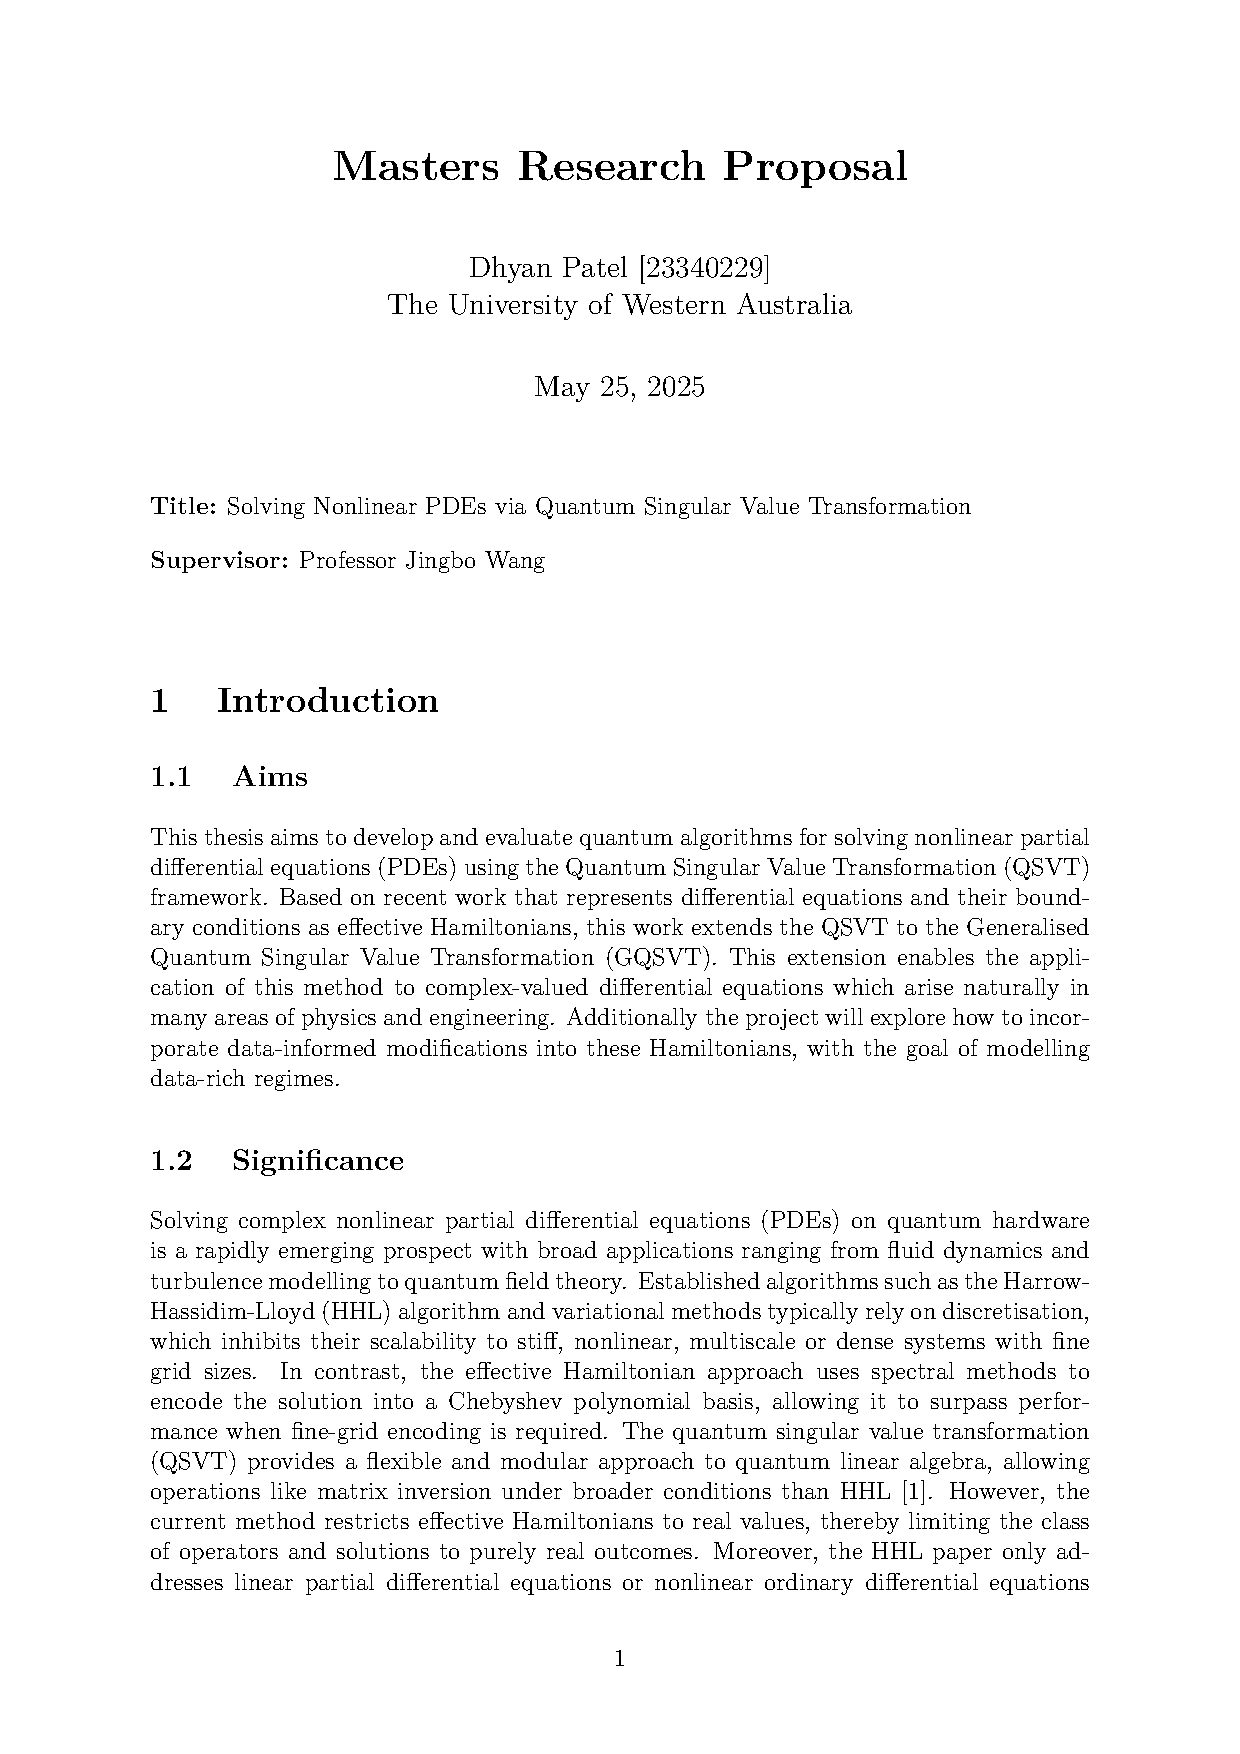
\includepdf[pages=-, scale=0.9, pagecommand={\thispagestyle{plain}}]{3_footer/research_proposal.pdf}
